
%------------DOC TYPE-------------------%
\documentclass[10pt]{article}

%-----------INCLUDES----------------------%
\usepackage[english]{babel}
\usepackage[utf8x]{inputenc}
\usepackage[left=2.5cm, right=2cm, top=2.5cm]{geometry} %margins
\usepackage{amsmath}
\usepackage{graphicx}
\usepackage[colorinlistoftodos]{todonotes}
\usepackage{subfiles}
\usepackage{titlesec}
\usepackage{fancyhdr}
\usepackage{verbatim}
\usepackage[bottom]{footmisc}
\usepackage{float} %CONCRETE FIGURE PLACEMENT
\usepackage{listings} %CODE LISINGS
\usepackage{color}
\usepackage{tikzit}
\usepackage{bm}
\usepackage{tabu}
\usepackage{hhline}
\usepackage[T1]{fontenc}
\usepackage[utf8x]{inputenc}
\usepackage[english]{babel}
\usepackage{csvsimple}
\usepackage{hyperref}
\usepackage{epsfig}
\usepackage{makecell}
\usepackage{array}
\usepackage{xcolor,colortbl}
\usepackage{fixltx2e}
\usepackage{caption}
\usepackage{subcaption}
\usepackage{etoolbox}
%\usepackage{pgflibraryarrows}

\makeatletter
\patchcmd{\@verbatim}
  {\verbatim@font}
  {\verbatim@font\small}
  {}{}
\makeatother

%----------------TIKZ STYLES---------------%
%\input{3-CommsIP/figs/ptpStyle.tikzstyles}

\setcounter{secnumdepth}{2}

%---------------PAGE STYLE/HEADER-FOOTER-------------------%
\pagestyle{fancy}% Change page style to fancy
\fancyhf{}% Clear header/footer
\fancyhead[R]{2127147b}
%\fancyhead[L]{}
\fancyfoot[R]{\thepage}% \fancyfoot[R]{\thepage}
\renewcommand{\headrulewidth}{0.5pt}
\renewcommand{\footrulewidth}{0.5pt}
\fancypagestyle{plain}{} %put HF on chapter page
 
 % footnote in footer
\renewcommand*\footnoterule{}
 
%-------------TITLE CONFIG--------%
%\titleformat{\chapter}[display]
 % {\normalfont\bfseries}{}{0pt}{\LARGE}

 %-----------FONT--------------%
 %\renewcommand{\familydefault}{ptm}

%-----------GRAPHICS---------------%
\graphicspath{{../figures/}}
\input{control5.tikzstyles}
\newcommand{\graphScale}{0.4}
\newcommand{\bigScale}{0.6}
%-------TABLES----------%
\newcolumntype{?}{!{\vrule width 1pt}}

\definecolor{jamie}{rgb}{1,1,0.82}
\newcommand{\done}{\cellcolor{jamie}done}  %{0.9}
\newcommand{\hcyan}[1]{{\color{teal} #1}}

%-------LISTINGS----------%
\definecolor{codegreen}{rgb}{0,0.6,0}
\definecolor{codegray}{rgb}{0.5,0.5,0.5}
\definecolor{codepurple}{rgb}{0.58,0,0.82}
\definecolor{backcolour}{rgb}{0.95,0.95,0.92}
 
\lstdefinestyle{mystyle}
{
    backgroundcolor=\color{backcolour},   
    commentstyle=\color{codegreen},
    keywordstyle=\color{blue},
    numberstyle=\tiny\color{codegray},
    stringstyle=\color{codepurple},
    basicstyle=\ttfamily\footnotesize,
    breakatwhitespace=false,         
    breaklines=true,                 
    captionpos=b,                    
    keepspaces=true,                 
    numbers=left,                    
    numbersep=5pt,                  
    showspaces=false,                
    showstringspaces=false,
    showtabs=false,                  
    tabsize=1
}


\lstset
{
    emph={BYTE_SWAP},
    emphstyle={\color{orange}},
    otherkeywords = {memset, memcpy},
    style=mystyle
}

\providecommand{\main}{.}

%------------STRUCTURE------------%
\begin{document}

\title{Advanced Control 5 (ENG5009) \\ \large{Lab Assignment}}
\author{2127147b}
\maketitle

\begin{abstract}
    \addcontentsline{toc}{chapter}{Abstract}
    The following report outlines the development and testing of a waypoint following and obstacle avoidance system for the simulation of an autonomous robot in MATLAB.
    The system presented uses fuzzy logic controllers to generate desired turning commands and motor gains. 
    A range of different input types were used alongside basic signal processing techniques to provide the fuzzy controllers with sufficient insight into the surrounding environment.
    The controller was found to produce successful results with the robot travelling to a specific coordinate within 0.05m. 
    Further development and fine-tuning was carried out to optimise the controller performance for a set of different scenarios.
    All code can be found on GitHub at \cite{github}, relevant code is included in the appendices.  
    \end{abstract}

\section{Methodology}
\subsection{Overview of System}
Two cascaded fuzzy controllers are used, the first (path controller) determines a desired turn command based solely on the robot's current heading angle ($\psi$) and its angle relative to a desired waypoint ($\psi_{ref}$).
The second controller takes the generated turn command with inputs relating to a nearby object ($d_{wall}$, $\bar{d}_{wall}$, $\Theta_{wall}$, $r$) to determine appropriate gains for the left and right motors.
A variable lowpass Finite Impulse Response (FIR) filter is used for each motor gain output to smooth the voltages, its cutoff frequency is controlled by one of the fuzzy motor controller outputs.
A proportional drive voltage is applied to each motor that varies with the robot's distance from the waypoint, it remains constant until close to the waypoint. 
A block diagram of the system can be seen in figure \ref{fig:system}.

\begin{figure}[H]
    \centering
    \ctikzfig{./figures/SystemDiagram}
    \caption{Block Diagram of Control System}
    \label{fig:system}
\end{figure}



\subsection{Task 1: Waypoint Following}
\subsubsection{Overview}
The aim of this task is to guide the robot to a set waypoint without obstacle avoidance.
This was achieved using fuzzy logic to generate a desired turn command by comparing the robot's current heading angle ($\psi$) with its angle relative to the waypoint ($\psi_{ref}$).
The fuzzy logic is implemented to drive the error between both angles to zero such that the robot travels in the direction of the waypoint.
 
\medskip
A second fuzzy controller was created to control the gain applied to the motors, it takes the generated turn command and radius from the waypoint as inputs.
As the robot approaches the waypoint, the rules are altered to enable coarser manoeuvres allowing it to stop within a 0.05m tolerance.
A drive voltage is also proportionally reduced as the robot's position converges on the waypoint. 

\subsubsection{Fuzzy Sets}

The input variables to the path controller are the heading and reference angles, they are measured from 0 rads (north), to either $-\pi$ or $+\pi$ rads (south) where a negative angle represents a counterclockwise angle and vice versa.
Nine fuzzy input sets were derived as follows, \{S\textsubscript{-ve}, SW, W, NW, N, NE, E, SE, S\textsubscript{+ve}\}, where N is north, NE is north-east etc, these sets are identical for both the heading and reference angle inputs.
S\textsubscript{-ve} and S\textsubscript{+ve} both represent a range around south as the angle jumps from -$\pi$ to $+\pi$ and are therefore treated as the same set in the fuzzy rules. 
Trapezoidal membership functions were used for fuzzification, they can be seen for the heading angle input in figure \ref{fig:headingSets}, the sets for the reference angle input are identical.

\begin{figure}[H]
    \centering
\includegraphics[scale=\graphScale]{./figures/HeadingControlInput2.eps}
\caption{Membership Functions for Heading Angle Input}
\label{fig:headingSets}
\end{figure}

The path controller output variable is a turning command with the derived set, 
\{L\textsubscript{rev}, L\textsubscript{rot}, L\textsubscript{hard}, L\textsubscript{soft}, FWD, R\textsubscript{soft}, R\textsubscript{hard}, R\textsubscript{rot}, R\textsubscript{rev}\},
for reverse, rotate, hard, soft and forward manoeuvres respectively. 
These commands allow for a variety of coarse or fine turning adjustments to be made by the motor controller, trapezoidal membership functions were used for the fuzzification and can be seen in figure \ref{fig:commandSets}
\begin{figure}[H]
    \centering
\includegraphics[scale=\graphScale]{./figures/HeadingControlOutput1.eps}
\caption{Membership Functions for Turn Command Output}
\label{fig:commandSets}
\end{figure}

The second input to the motor controller is the robot's radius to the waypoint with the following set, \{VN, N, F, VF\}, representing very-near, near, far and very-far respectively.
This is used to execute tighter turning manoeuvres when close to the waypoint as when the robot is very-near to the waypoint, the turn command will begin to change much more rapidly.
This therefore needs to be taken into account such that the robot can navigate to within 0.05m.
The radius is also used in the main code to proportionally reduce the drive voltage on approach to the waypoint.
Trapezoidal membership functions are used and can be seen in figure \ref{fig:radiusSets}.

\begin{figure}[H]
    \centering
\includegraphics[scale=\graphScale]{./figures/MotorControlInput2.eps}
\caption{Membership Functions for Radius Input}
\label{fig:radiusSets}
\end{figure}

The motor controller produces gains for the motors as outputs in the range of -1 to 1 with the derived set, \{REV\textsubscript{hard}, REV\textsubscript{soft}, OFF, FWD\textsubscript{soft}, FWD\textsubscript{hard}\},
representing hard-reverse, soft-reverse, off, soft-forward and hard-forward manoeuvres repectively. 
These gains are scaled in the main code to an appropriate range and limited to the maximum range of $\pm$7.4V. 
Triangular membership functions are used and can be seen in figure \ref{fig:motorSets}.


\begin{figure}[H]
    \centering
\includegraphics[scale=\graphScale]{./figures/MotorControlOutput1.eps}
\caption{Membership Functions for Motor Gain Outputs}
\label{fig:motorSets}
\end{figure}

\subsubsection{Rules}
The path controller will produce a turning command that is appropriate for the robot's heading in relation to the its reference angle to the waypoint.
For example: \textbf{IF} the robot is facing north ($\psi$=N) \textbf{AND} its bearing is north east ($\psi_{ref}$=NE), \textbf{THEN} turn soft right (R\textsubscript{soft}).
In this situation only a soft right turn is required as angles in north and north-east are likely to be close together, a harder manoeuvre is more likely to result in an undesired overshoot.
Rules were derived for each combination of headings and reference angles, a sample of the 81 rules can be seen in table \ref{table:cmdRules} for a heading angle of south-positive.
The defuzzification method used was the bisector method.
The entire set of rules are included in appendix ???????????????????.

\begin{table}[H]
    \centering  
    \caption{Sample of Fuzzy Logic Rules for Path Controller (outputs in yellow)}
    \begin{tabu} to 0.8\textwidth { ? l | l ? l ? l ?}
        \Xhline{2\arrayrulewidth}
        $\psi_{ref}$   & $\psi$ &  \cellcolor{jamie} \textbf{TURN CMD} \\
        %\hhline{|=|=||=|}
        \Xhline{2\arrayrulewidth}
        S\textsubscript{-ve}  &  S\textsubscript{-ve}  &\cellcolor{jamie} FWD\\
        \hline
        S\textsubscript{-ve}  &  SW &\cellcolor{jamie} L\textsubscript{soft}\\ 
        \hline
        S\textsubscript{-ve}  &  W &\cellcolor{jamie} L\textsubscript{hard}\\
        \hline
        S\textsubscript{-ve}  & NW&\cellcolor{jamie} L\textsubscript{rot}\\
        \hline
        S\textsubscript{-ve}  &  N&\cellcolor{jamie} L\textsubscript{rev}\\
        \hline
        S\textsubscript{-ve}  & NE & \cellcolor{jamie} R\textsubscript{rot}\\
        \hline
        S\textsubscript{-ve}  & E & \cellcolor{jamie} R\textsubscript{hard}\\
        \hline 
        S\textsubscript{-ve}  & SE & \cellcolor{jamie} R\textsubscript{soft}\\
        \hline
        S\textsubscript{-ve}   & S\textsubscript{+ve}  & \cellcolor{jamie} FWD\\

        \Xhline{2\arrayrulewidth}
    \end{tabu}
    
    \label{table:cmdRules}
\end{table}

The motor controller interprets these turn commands by applying appropriate gains to the left and right motors such that robot executes the requested turning manoeuvre.
For example: \textbf{IF} the requested manoeuvre is a soft-right turn (TURN CMD = R\textsubscript{soft}) \textbf{AND} the robot is not very-near to the waypoint ($r$ != VN), \textbf{THEN} $A_{left}$ is FWD\textsubscript{soft} \textbf{AND} $A_{left}$ is OFF.
If the robot is very-near to the waypoint then it will only execute rotational manoeuvres, for example:
\textbf{IF} the requested manoeuvre is a soft-right turn \textbf{AND} the robot is very-near ($r$ = VN), \textbf{THEN} $A_{left}$ is FWD\textsubscript{soft} \textbf{AND} $A_{left}$ is REV\textsubscript{soft}.

These rules can be seen in table \ref{table:motorOut1}

\begin{table}[H]
    \centering  
    \caption{Truth table of motor controller rules (outputs in yellow)}
    \begin{tabu} to 0.8\textwidth { ? l | l | l | l ?}
        \Xhline{2\arrayrulewidth}
        \textbf{TURN CMD}   & $r$  &\cellcolor{jamie} $A_{left}$ & \cellcolor{jamie} $A_{right}$ \\
        %\hhline{|=|=||=|}
        \Xhline{2\arrayrulewidth}
        FWD  &  !VN &                              \cellcolor{jamie} FWD\textsubscript{soft} & \cellcolor{jamie} FWD\textsubscript{soft} \\
        \hline
        L\textsubscript{soft} &!VN   &            \cellcolor{jamie} OFF &          \cellcolor{jamie}FWD \textsubscript{soft} \\ 
        \hline
        L\textsubscript{hard} &!VN   &             \cellcolor{jamie} REV\textsubscript{soft} &          \cellcolor{jamie}FWD \textsubscript{hard} \\ 
        \hline
        L\textsubscript{rot}& !VN &             \cellcolor{jamie} REV\textsubscript{hard}&\cellcolor{jamie}FWD \textsubscript{hard}\\
        \hline
        L\textsubscript{rev} &  !VN &             \cellcolor{jamie} REV\textsubscript{hard}&\cellcolor{jamie}REV\textsubscript{soft}\\
        \hline
        R\textsubscript{rev} & !VN &             \cellcolor{jamie} REV\textsubscript{soft}&\cellcolor{jamie}REV\textsubscript{hard}\\
        \hline
        R\textsubscript{rot} & !VN &             \cellcolor{jamie} FWD\textsubscript{hard}&\cellcolor{jamie}REV\textsubscript{hard}\\
        \hline 
        R\textsubscript{hard}& !VN&              \cellcolor{jamie} FWD\textsubscript{hard}&\cellcolor{jamie}REV\textsubscript{soft}\\
        \hline
        R\textsubscript{soft}  & !VN &             \cellcolor{jamie} FWD\textsubscript{soft}&\cellcolor{jamie}OFF\\

        \hline
        FWD  &  VN &                            \cellcolor{jamie} FWD\textsubscript{soft}&\cellcolor{jamie}FWD\textsubscript{soft}\\
        \hline
        L\textsubscript{soft} &VN   &          \cellcolor{jamie} REV\textsubscript{soft}&\cellcolor{jamie}FWD\textsubscript{soft}\\
        \hline
        L\textsubscript{hard} &VN    &           \cellcolor{jamie} REV\textsubscript{hard}&\cellcolor{jamie}FWD\textsubscript{hard}\\
        \hline
        L\textsubscript{rot}& VN     &            \cellcolor{jamie} REV\textsubscript{hard}&\cellcolor{jamie}FWD\textsubscript{hard}\\
        \hline
        L\textsubscript{rev} &  VN &              \cellcolor{jamie} REV\textsubscript{hard}&\cellcolor{jamie}FWD\textsubscript{hard}\\
        \hline
        R\textsubscript{rev} & VN &         \cellcolor{jamie} FWD\textsubscript{hard}&\cellcolor{jamie}REV\textsubscript{hard}\\
        \hline
        R\textsubscript{rot} & VN &              \cellcolor{jamie} FWD\textsubscript{hard}&\cellcolor{jamie}REV\textsubscript{hard}\\
        \hline 
        R\textsubscript{hard}& VN&             \cellcolor{jamie} FWD\textsubscript{hard}&\cellcolor{jamie}REV\textsubscript{hard}\\
        \hline
        R\textsubscript{soft}  & VN &             \cellcolor{jamie} FWD\textsubscript{soft}&\cellcolor{jamie}REV\textsubscript{soft}\\

        \Xhline{2\arrayrulewidth}
    \end{tabu}
    
    \label{table:motorOut1}
    \end{table}

\subsubsection{Verification}
The path controller was tested using the waypoints specified in the assignment brief (task 1). 
The results shown in table \ref{table:task1} demonstrate that the testing was successful as the robot stopped at a point within 0.05m of the waypoint in each scenario.
An example plot of the robot's path from the origin to (-0.2, 2) is shown in figure \ref{fig:task1}.

\begin{table}[H]
    \centering  
    \caption{Start and end coordinates for task 1}
    \begin{tabu} to 0.8\textwidth { ? l | l ?}
        \Xhline{2\arrayrulewidth}
        \textbf{Start Coordinate}  &  \textbf{End Coordinate}\\
        %\hhline{|=|=||=|}
        \Xhline{2\arrayrulewidth}
        (0, 3) & (-0.043, 3.0246) \\
        \hline
        (1, 2) & (0.9949, 2.0463) \\
        \hline
        (-1, 4) & (-1.0409, 4.0230) \\
        \hline
        (-1, 2) & (-1.0448, -1.9871) \\
        \hline
        (0, 3) & (-0.2391, 2.0056) \\
        \Xhline{2\arrayrulewidth}
    \end{tabu}
    
    \label{table:task1}
    \end{table}

    \begin{figure}[H]
        \centering
    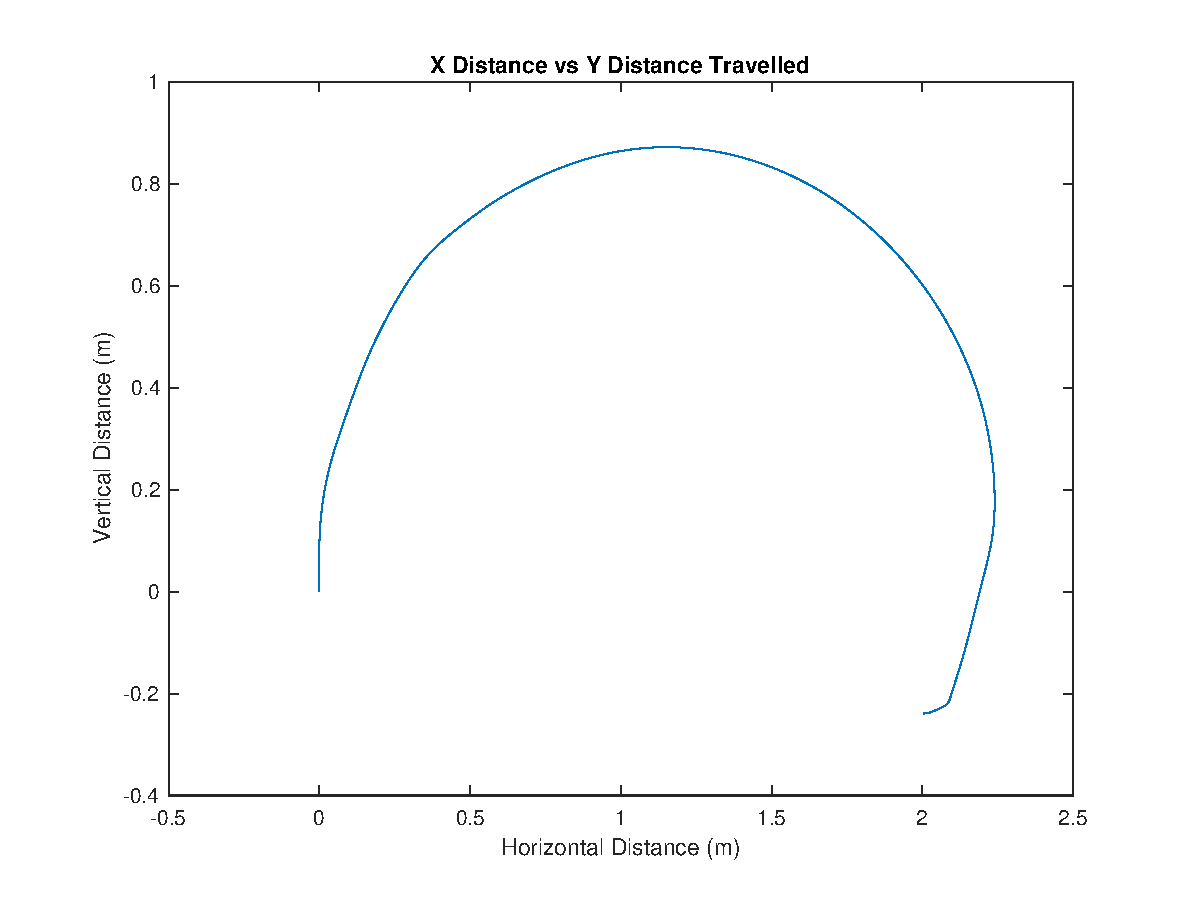
\includegraphics[scale=\graphScale]{./figures/task1_x0point2y2.eps}
    \caption{Path of robot from the origin to (-0.2, 2)}
    \label{fig:task1}
    \end{figure}

\subsection{Task 2: Obstacle Avoidance}

\subsubsection{Overview}
The aim of this task is to guide the robot to a set waypoint as before, however doing so while avoiding obstacles.
This was achieved using additional inputs from distance sensors to the motor controller such that the robot could execute evasive manoeuvres when in the proximity of a wall.
The fuzzy logic is implemented in such a way as to drive the error between the heading and reference angles to zero (as in task one) when outwith the proximity of a wall however, different evasion commands would be executed as required when near a wall.

\subsubsection{Fuzzy Sets}
%INPUTS
The angle at which the robot approaches an obstacle ($\Theta_{wall}$) is an input to the motor controller and is calculated in the main code using the following equation:
$\Theta = arctan\bigg(\frac{d_{left}-d_{right}}{\Delta x}\bigg)$,
where $d_{left}$, $d_{right}$ and $\Delta x$ are the left sensor distance, right sensor distance and distance between the sensors respectively.
As the maximum output from a sensor is 1 and the distance between the sensors is 0.2, the maximum detectable wall angle/slope is 1.3734 and therefore the range of the fuzzy input set is $\pm$1.3734.
The derived set is as follows, \{-ve\textsubscript{hard}, -ve\textsubscript{soft}, FLAT, +ve\textsubscript{soft}, +ve\textsubscript{hard}\}, where each member represents a slope gradient.

\medskip
For example, -ve\textsubscript{hard} refers to a steep negative gradient relative to the direction that the robot is facing the wall.
This set uses trapezoidal membership functions for all but the FLAT member, it was found that the controller performed best when limiting the FLAT member to a small range with a triangular function as otherwise it would become indecisive when approaching the wall at a slight angle in certain scenarios. 
These can be seen in figure \ref{fig:wallSlope}.
\begin{figure}[H]
    \centering
\includegraphics[scale=\graphScale]{./figures/MotorControlInput3.eps}
\caption{Membership Functions for Wall Angle Input}
\label{fig:wallSlope}
\end{figure}

The proximity to the wall is determined as the smaller of either distances detected by the left or right sensors and is an input with the following set, \{CLOSE, NEAR, FAR\} with trapezoidal membership functions that can be seen in figure \ref{fig:wallProx}.
Since the sensor returns one when an obstacle is not detected, any input greater than this is definitively a FAR value of proximity as this allows the controller logic to function reliably when detecting a wall. 
The controller is designed to guide the robot alongside the wall until it reaches its corner, at which point it can continue towards the waypoint as normal.

\begin{figure}[H]
    \centering
\includegraphics[scale=\graphScale]{./figures/MotorControlInput4.eps}
\caption{Membership Functions for Wall Proximity Input}
\label{fig:wallProx}
\end{figure}

In certain situations the robot will begin tracking along a wall with the waypoint initially directly on the other side. 
As it moves along the wall, the difference between the heading and reference angles begins to increase and therefore, the requested turning command will become more aggressive. 
This becomes a problem when the robot is in parallel with the wall as its sensors return a value of one and thus the robot acts as though it is FAR from the wall.
In this situation, when the turning command is aggressive, the robot will jolt towards the wall as soon as it becomes parallel. 

\medskip
To rectify this, it was necessary to provide the controller with an input that could indicate whether or not the robot had cleared a wall while tracking along it. 
This was achieved by taking a 20 sample moving average (mean) of the wall proximity and providing this as an additional input ($\bar{d}_{wall}$), the robot could be assumed to have cleared a wall only when both the filtered and unfiltered proximity values are one.
The fuzzy set and membership functions are identical to that of the unfiltered proximity seen in figure \ref{fig:wallProx}.

\medskip
A variable, Finite Impulse Response (FIR) lowpass filter was applied to smooth the output voltages.
This was achieved by writing and using a sample by sample FIR filter class, this can be seen in appendix ?????????.
Its cutoff frequency is an output of the motor controller such that the motor responsiveness could be adjusted dynamically in certain scenarios, its set is as follows, \{SLOW, AVG, FAST\}.
Trapezoidal membership function are used and can be seen in figure \ref{fig:filterOut}, its total range is from 0 to 1 as the filter is normalised to the nyquist frequency. 

%OUTPUTS


\begin{figure}[H]
    \centering
\includegraphics[scale=\graphScale]{./figures/MotorControlOutput3.eps}
\caption{Membership Functions for Filter Cutoff Frequency Output}
\label{fig:filterOut}
\end{figure}

\subsubsection{Rules}
When the robot is far from a wall and has cleared it in the situation that it was tracking alongside one, then it applies the same turn command that of task one in table \ref{table:cmdRules}.
When in proximity of a wall, an appropriate manoeuvre is executed to alter the robot such that it is in parallel with the wall depending on the wall angle relative to the robots heading. 
For example, \textbf{IF} the robot is facing the wall with a steep positive gradient ($\Theta_{wall}$ = +ve\textsubscript{hard}) \textbf{AND} the robot is NEAR to the wall, \textbf{THEN} $A_{left}$ is FWD\textsubscript{hard} \textbf{AND} $A_{right}$ is FWD\textsubscript{soft}.
In this scenario, the robot is close to parallel to the wall so only a gentle right turn is required.
In situations where the robot approaches the wall at a flat angle, the robot will turn left or right depending on the current turn command requested by the path controller, if the turn command requested is forward the robot will turn right by default.
This can be seen in table \ref{table:wallProxRules}. 

\begin{comment}
\begin{table}[H]
    \centering  
    \caption{Truth table of motor controller rules when outwidth the proximity of a wall}
    \begin{tabu} to 0.8\textwidth { ? l | l | l | l | l ? l | l | l ?}
        \Xhline{2\arrayrulewidth}
        \textbf{TURN CMD}   & $r$ & $\Theta_{wall}$ &  $d_{wall}$ & $\bar{d}_{wall}$ &\cellcolor{jamie} $A_{left}$ & \cellcolor{jamie} $A_{right}$ & \cellcolor{jamie} $\omega_{cut}$\\
        %\hhline{|=|=||=|}
        \Xhline{2\arrayrulewidth}
        FWD  &  !VN & X&FAR &FAR &                              \cellcolor{jamie} FWD\textsubscript{soft} & \cellcolor{jamie} FWD\textsubscript{soft} & \cellcolor{jamie} AVG\\
        \hline
        L\textsubscript{soft} &!VN   &X& FAR&FAR &              \cellcolor{jamie} OFF &          \cellcolor{jamie}FWD \textsubscript{soft} & \cellcolor{jamie}AVG\\ 
        \hline
        L\textsubscript{hard} &!VN   &X& FAR&FAR &              \cellcolor{jamie} REV\textsubscript{soft} &          \cellcolor{jamie}FWD \textsubscript{hard} & \cellcolor{jamie}AVG\\ 
        \hline
        L\textsubscript{rot}& !VN &X& FAR&FAR &                 \cellcolor{jamie} REV\textsubscript{hard}&\cellcolor{jamie}FWD \textsubscript{hard}&\cellcolor{jamie}AVG\\
        \hline
        L\textsubscript{rev} &  !VN &X& FAR&FAR &               \cellcolor{jamie} REV\textsubscript{hard}&\cellcolor{jamie}REV\textsubscript{soft}&\cellcolor{jamie}AVG\\
        \hline
        R\textsubscript{rev} & !VN &X& FAR& FAR&                \cellcolor{jamie} REV\textsubscript{soft}&\cellcolor{jamie}REV\textsubscript{hard}&\cellcolor{jamie}AVG\\
        \hline
        R\textsubscript{rot} & !VN & X& FAR&FAR &               \cellcolor{jamie} FWD\textsubscript{hard}&\cellcolor{jamie}REV\textsubscript{hard}&\cellcolor{jamie}AVG\\
        \hline 
        R\textsubscript{hard}& !VN&X& FAR&FAR &                 \cellcolor{jamie} FWD\textsubscript{hard}&\cellcolor{jamie}REV\textsubscript{soft}&\cellcolor{jamie}AVG\\
        \hline
        R\textsubscript{soft}  & !VN &X& FAR& FAR&              \cellcolor{jamie} FWD\textsubscript{soft}&\cellcolor{jamie}OFF&\cellcolor{jamie}AVG\\

        \hline
        FWD  &  VN & X&FAR &FAR &                               \cellcolor{jamie} FWD\textsubscript{soft}&\cellcolor{jamie}FWD\textsubscript{soft}&\cellcolor{jamie}AVG\\
        \hline
        L\textsubscript{soft} &VN   &X& FAR&FAR &               \cellcolor{jamie} REV\textsubscript{soft}&\cellcolor{jamie}FWD\textsubscript{soft}&\cellcolor{jamie}AVG\\
        \hline
        L\textsubscript{hard} &VN   &X& FAR&FAR &               \cellcolor{jamie} REV\textsubscript{hard}&\cellcolor{jamie}FWD\textsubscript{hard}&\cellcolor{jamie}AVG\\
        \hline
        L\textsubscript{rot}& VN &X& FAR&FAR &                  \cellcolor{jamie} REV\textsubscript{hard}&\cellcolor{jamie}FWD\textsubscript{hard}&\cellcolor{jamie}AVG\\
        \hline
        L\textsubscript{rev} &  VN &X& FAR&FAR &                \cellcolor{jamie} REV\textsubscript{hard}&\cellcolor{jamie}FWD\textsubscript{hard}&\cellcolor{jamie}AVG\\
        \hline
        R\textsubscript{rev} & VN &X& FAR& FAR&                 \cellcolor{jamie} FWD\textsubscript{hard}&\cellcolor{jamie}REV\textsubscript{hard}&\cellcolor{jamie}AVG\\
        \hline
        R\textsubscript{rot} & VN & X& FAR&FAR &                \cellcolor{jamie} FWD\textsubscript{hard}&\cellcolor{jamie}REV\textsubscript{hard}&\cellcolor{jamie}AVG\\
        \hline 
        R\textsubscript{hard}& VN&X& FAR&FAR &                  \cellcolor{jamie} FWD\textsubscript{hard}&\cellcolor{jamie}REV\textsubscript{hard}&\cellcolor{jamie}AVG\\
        \hline
        R\textsubscript{soft}  & VN &X& FAR& FAR&               \cellcolor{jamie} FWD\textsubscript{soft}&\cellcolor{jamie}REV\textsubscript{soft}&\cellcolor{jamie}AVG\\

        \Xhline{2\arrayrulewidth}
    \end{tabu}
    
    \label{table:IPfuncs}
    \end{table}
\end{comment}

%wall avoidance
\begin{table}[H]
    \centering  
    \caption{Truth table of motor controller rules when within proximity of a wall}
    \begin{tabu} to 0.8\textwidth { ? l | l | l | l | l ? l | l | l ?}
        \Xhline{2\arrayrulewidth}
        \textbf{TURN CMD}   & $r$ & $\Theta_{wall}$ &  $d_{wall}$ & $\bar{d}_{wall}$ &\cellcolor{jamie} $A_{left}$ & \cellcolor{jamie} $A_{right}$ & \cellcolor{jamie} $\omega_{cut}$\\
        %\hhline{|=|=||=|}
        \Xhline{2\arrayrulewidth}
    
        X & X & +ve\textsubscript{hard} & NEAR & X &             \cellcolor{jamie} FWD\textsubscript{hard}&\cellcolor{jamie}FWD\textsubscript{soft}&\cellcolor{jamie}AVG\\
        \hline
        X & X & +ve\textsubscript{soft} & NEAR & X &             \cellcolor{jamie} FWD\textsubscript{hard}&\cellcolor{jamie}REV\textsubscript{soft}&\cellcolor{jamie}AVG\\
        \hline 
        X & X & +ve\textsubscript{hard} & CLOSE & X &             \cellcolor{jamie} FWD\textsubscript{hard}&\cellcolor{jamie}FWD\textsubscript{soft}&\cellcolor{jamie}AVG\\
        \hline
        X & X & +ve\textsubscript{soft} & CLOSE & X &             \cellcolor{jamie} FWD\textsubscript{hard}&\cellcolor{jamie}REV\textsubscript{hard}&\cellcolor{jamie}AVG\\
        \hline
        X & X & -ve\textsubscript{hard} & NEAR & X &             \cellcolor{jamie} FWD\textsubscript{soft}&\cellcolor{jamie}FWD\textsubscript{hard}&\cellcolor{jamie}AVG\\
        \hline
        X & X & -ve\textsubscript{soft} & NEAR & X &             \cellcolor{jamie} REV\textsubscript{soft}&\cellcolor{jamie}FWD\textsubscript{hard}&\cellcolor{jamie}AVG\\
        \hline 
        X & X & -ve\textsubscript{hard} & CLOSE & X &             \cellcolor{jamie} FWD\textsubscript{soft}&\cellcolor{jamie}FWD\textsubscript{hard}&\cellcolor{jamie}AVG\\
        \hline
        X & X & -ve\textsubscript{soft} & CLOSE & X &             \cellcolor{jamie} REV\textsubscript{hard}&\cellcolor{jamie}FWD\textsubscript{hard}&\cellcolor{jamie}AVG\\




        \hline
        FWD  & X & FLAT & !FAR &X  &                               \cellcolor{jamie} FWD\textsubscript{hard}&\cellcolor{jamie}REV\textsubscript{soft}&\cellcolor{jamie}FAST\\
        \hline
        L\textsubscript{any} & X & FLAT & !FAR & X &               \cellcolor{jamie} REV\textsubscript{soft}&\cellcolor{jamie}FWD\textsubscript{hard}&\cellcolor{jamie}FAST\\
        \hline
        R\textsubscript{any} & X & FLAT & !FAR & X &               \cellcolor{jamie} FWD\textsubscript{hard}&\cellcolor{jamie}REV\textsubscript{soft}&\cellcolor{jamie}FAST\\

        \Xhline{2\arrayrulewidth}
    \end{tabu}
    
    \label{table:wallProxRules}
    \end{table}

%with filtered inputs (wall hugging)
When tracking along a wall, if the robot is parallel and the waypoint resides an the other side of it, the motor controller will execute a soft turning command towards the wall.
This prevents the the robot jolting towards the wall when an aggressive turning command is requested by the path controller as described previously.
The logic is implemented such that these rules are enabled when the unfiltered wall proximity is FAR but the unfiltered proximity is not, i.e. the robot is parallel and therefore still tracking along the wall.
This can be seen in figure \ref{table:parMotorRules}.

\begin{table}[H]
    \centering  
    \caption{Truth table of motor controller rules when approximately parallel to wall}
    \begin{tabu} to 0.8\textwidth { ? l | l | l | l | l ? l | l | l ?}
        \Xhline{2\arrayrulewidth}
        \textbf{TURN CMD}   & $r$ & $\Theta_{wall}$ &  $d_{wall}$ & $\bar{d}_{wall}$ &\cellcolor{jamie} $A_{left}$ & \cellcolor{jamie} $A_{right}$ & \cellcolor{jamie} $\omega_{cut}$\\
        %\hhline{|=|=||=|}
        \Xhline{2\arrayrulewidth}
    
        R\textsubscript{rev} & !VN & X & FAR & !FAR &               \cellcolor{jamie} FWD\textsubscript{hard}&\cellcolor{jamie}FWD\textsubscript{soft}&\cellcolor{jamie}AVG\\
        \hline
        R\textsubscript{rot} & !VN & X & FAR & !FAR &               \cellcolor{jamie} FWD\textsubscript{hard}&\cellcolor{jamie}FWD\textsubscript{soft}&\cellcolor{jamie}AVG\\
        \hline
        L\textsubscript{rev} & !VN & X & FAR & !FAR &               \cellcolor{jamie} FWD\textsubscript{soft}&\cellcolor{jamie}FWD\textsubscript{hard}&\cellcolor{jamie}AVG\\
        \hline
        L\textsubscript{rot} & !VN & X & FAR & !FAR &               \cellcolor{jamie} FWD\textsubscript{soft}&\cellcolor{jamie}FWD\textsubscript{hard}&\cellcolor{jamie}AVG\\

        \Xhline{2\arrayrulewidth}
    \end{tabu}
    
    \label{table:parMotorRules}
    \end{table}



\section{Results and Testing}
\subsubsection{Assigned Waypoint}
The following plot (figure \ref{fig:ToWaypoint}) shows the robot's path towards the waypoint specified in the assignment brief (3.5, 2.5).
The robot was successful in reaching the waypoint within a 0.05m tolerance, finishing at the coordinate (3.5342, 2.5302).
A subtle avoidance manoeuvre is executed as it reaches the wall at (1.2, -1), the robot tracks alongside the wall until it has cleared it at (1.2, 1) at which it point it turns left towards the waypoint.
As its position converges on that of the waypoint, a left rotation is executed demonstrating the successful execution of rules to be enabled when very-near to the waypoint. 
\begin{figure}[H]
    \centering
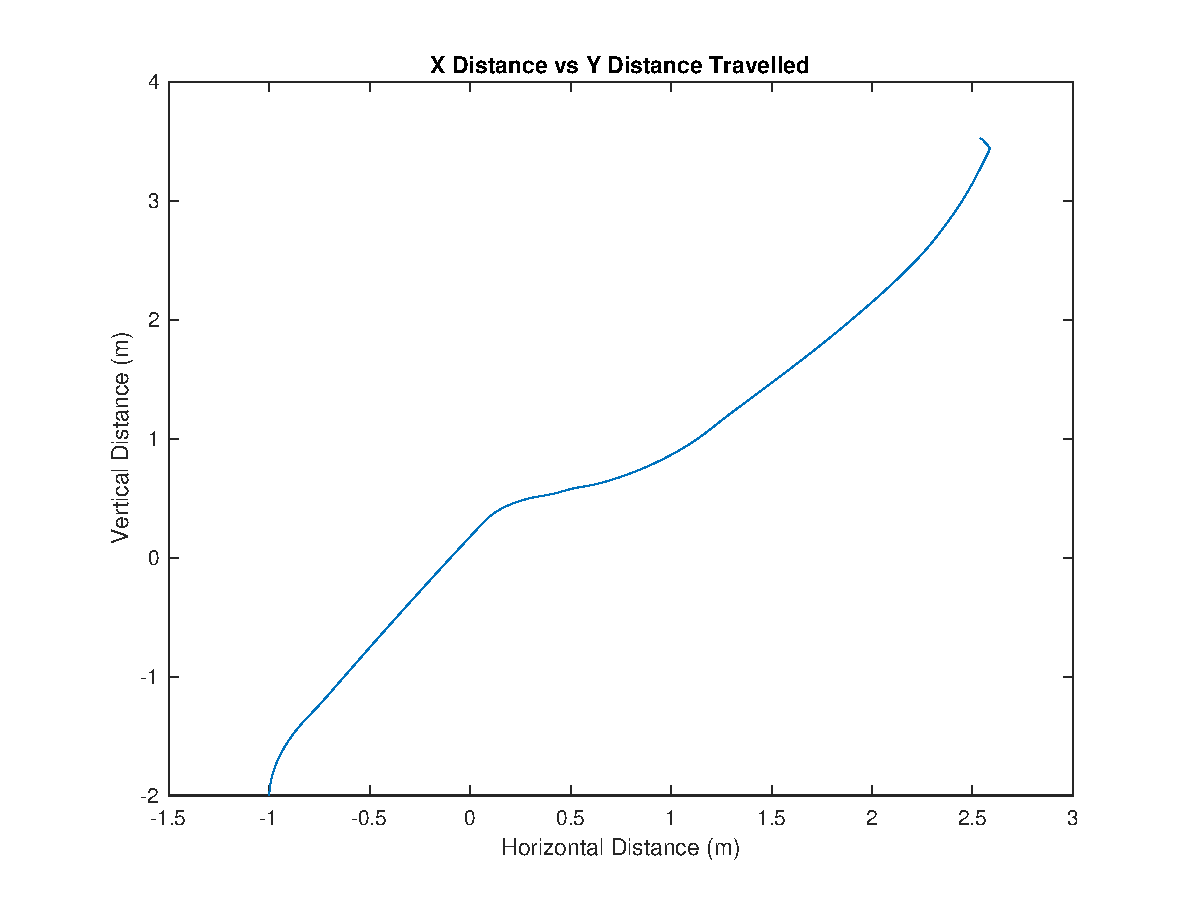
\includegraphics[scale=\graphScale]{./figures/ToWaypoint.eps}
\caption{Robot path to waypoint (3.5, 2.5) from starting point (-2, -1)}
\label{fig:ToWaypoint}
\end{figure}


\subsubsection{Wall Tracking}
%average filter
In order to test the robot's ability to detect whether or not it was in parallel to a wall, the following test scenario was devised.
The robot is initially directly facing a wall, the waypoint is placed directly opposite the robot on the other side of the wall.
The controller will guide the robot around the wall to the right, when the filtered proximity input is enabled the robot should track along the wall smoothly and when disabled, it should track in a jagged fashion.
This input was disabled by setting it as one, ensuring that the relevant rules would never fire. 
The results can be seen in figure \ref{fig:wallFilter}.
When the filtered proximity input is enabled (\ref{fig:filtSub2}), the path as the robot tracks along the wall is much smoother than when disabled (\ref{fig:filtSub1}).

\begin{figure}[H]
    \centering
    \begin{subfigure}{.5\textwidth}
      \centering
      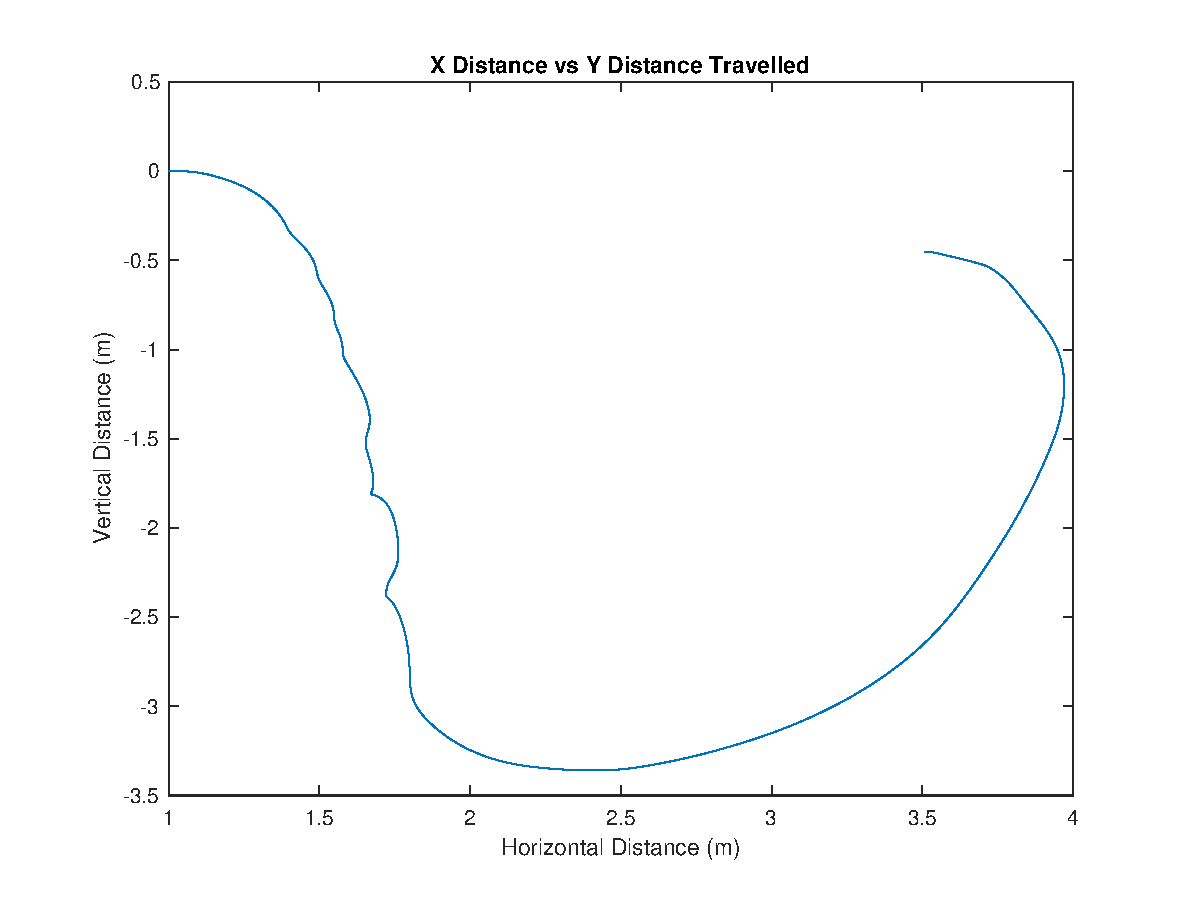
\includegraphics[scale=0.4]{./figures/SharpTurn_noFilt.eps}
      \caption{No filtered proximity input rules applied}
      \label{fig:filtSub1}
    \end{subfigure}%
    \begin{subfigure}{.5\textwidth}
      \centering
      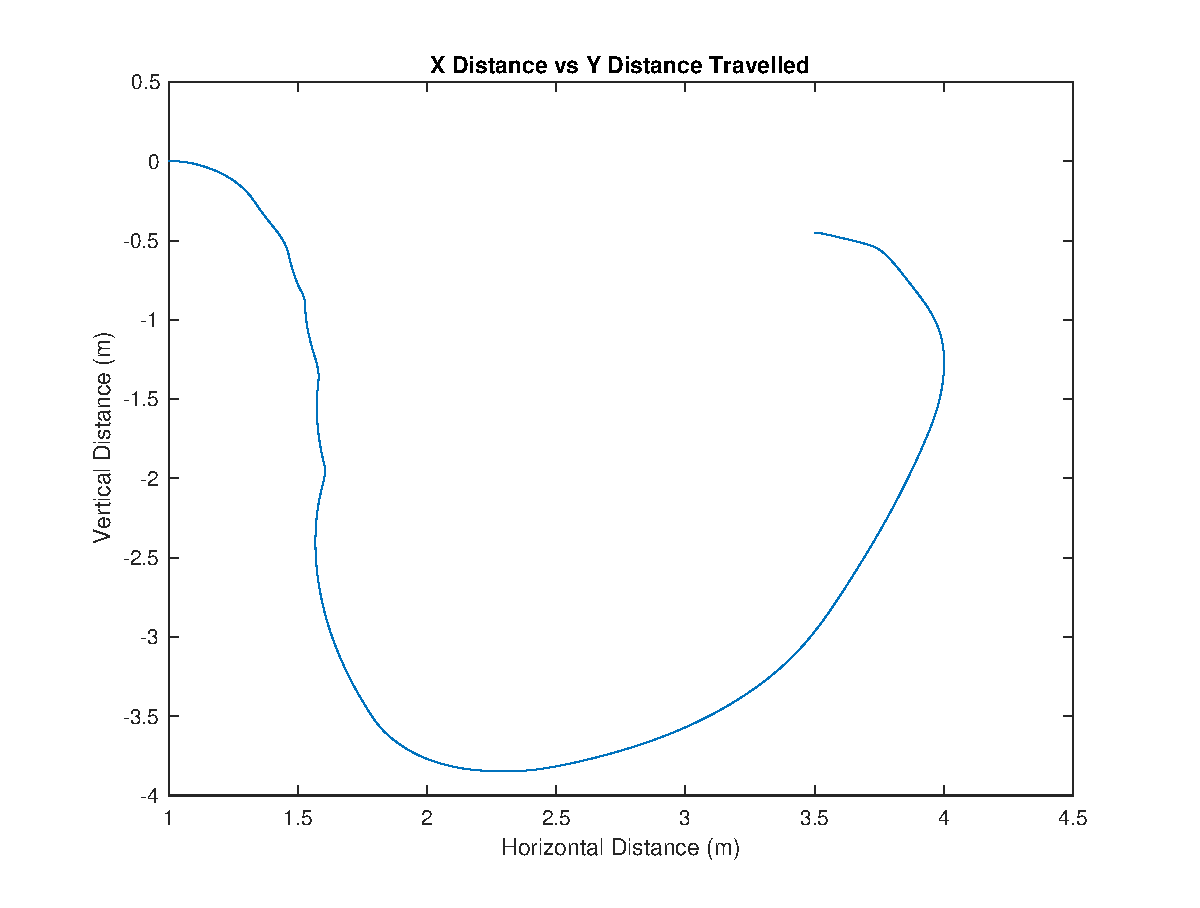
\includegraphics[scale=0.4]{./figures/SharpTurn_withFilt.eps}
      \caption{Filtered proximity input rules applied}
      \label{fig:filtSub2}
    \end{subfigure}
    \caption{Robot path with filtered proximity input}
    \label{fig:wallFilter}
    \end{figure}

\begin{comment}
\subsubsection{Perpendicular Approach}
%jolting, reducing flat member func
%filter
\begin{figure}[H]
    \centering
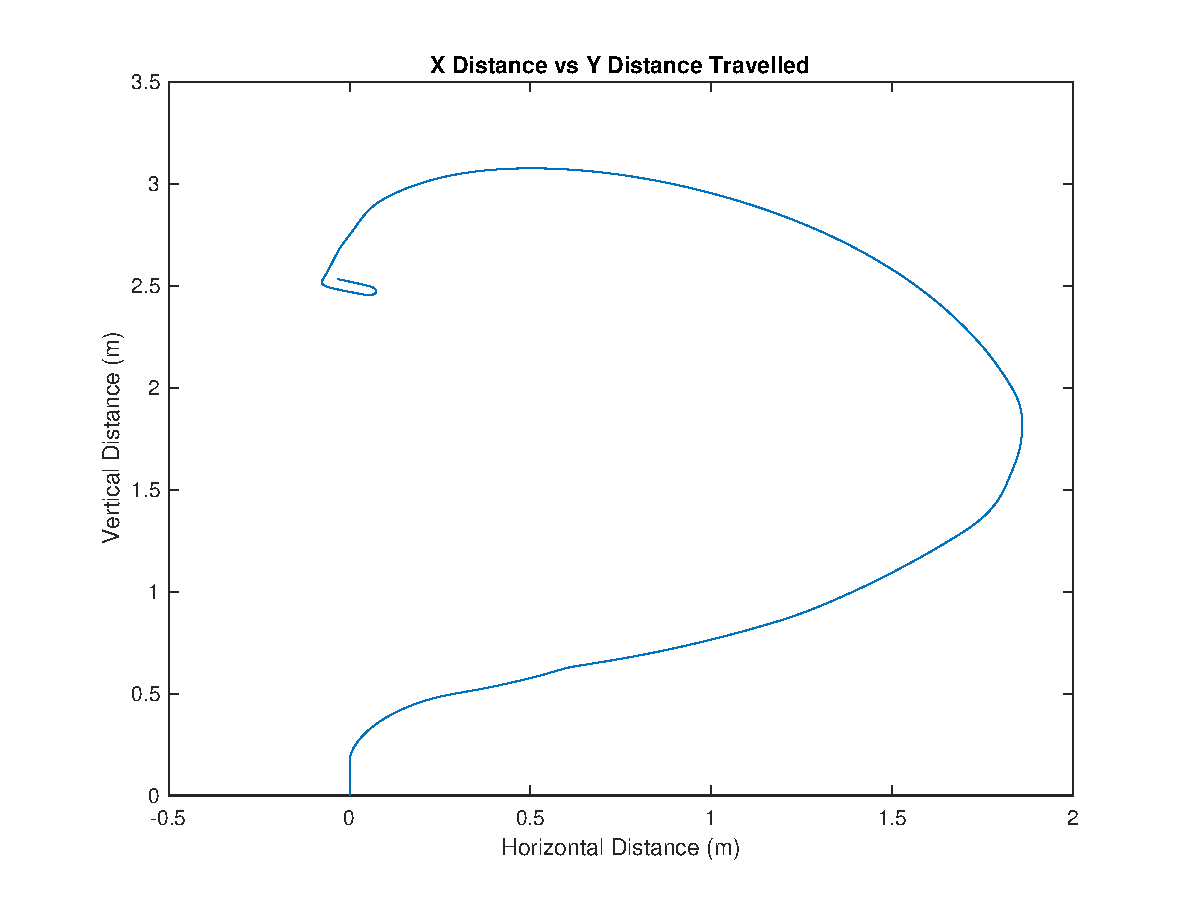
\includegraphics[scale=\graphScale]{./figures/PerpApproach.eps}
\caption{Path from (0, 2.5) to (0, 0) with perpendicular wall, (1.2, -1) to (1.2, 1)}
\end{figure}

\begin{figure}[H]
    \centering
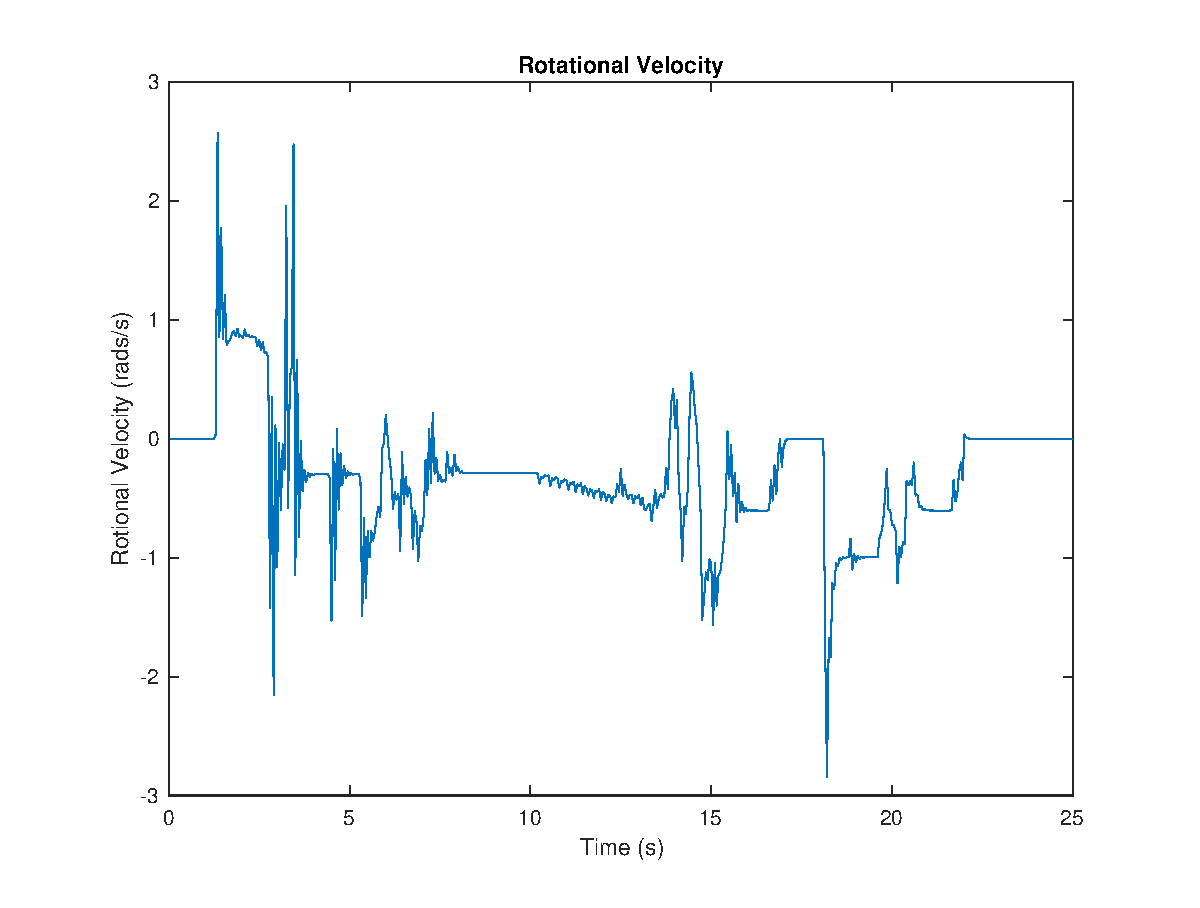
\includegraphics[scale=\graphScale]{./figures/PerpRotVel.eps}
\caption{Rotational velocity when avoiding a perpendicular wall}
\end{figure}
\end{comment}

\section{Further Work}
More rules need to be developed for waypoints residing close to a wall, the requested turn command will be ignored in such a scenario.
As the robot converges on the waypoint, it will come into proximity of the wall and the coarser turn commands, to be enabled when very-near to the waypoint, will not be fired resulting in the robot being unable to reach the point.
This could be rectified by adding further logic to account for the robot being near a wall AND the waypoint. 

\medskip
Simplifications could have been made to the logic to reduce unused or rarely used variables and members. 
The path controller's logic could have been simplified by calculating the error between the heading and reference angles and using this as a single fuzzy set, this would have resulted in only 9 rules rather than 81. 
The lowpass filter cutoff frequency is also rarely altered with the exception of the robot approaching a wall perpendicularly in which which it is increased to allow for a faster turning response.
More investigation should be done into how this output could be better utilised. 

\medskip
More fine-tuning to the motor controller rules could be carried out, particularly to those fired when close to the waypoint.
As can be seen in figure \ref{fig:ToWaypoint}, the robot stops abruptly next to the waypoint before rotating and approaching from a very small distance.
Ideally the trajectory as the robot approaches would be smoother and more gradual.
This could be achieved by adding more rules or members to the motor gain output set, increasing the potential resolution of the output voltages.  
%unused variables (velocity, rotational velocity)

\pagebreak
\bibliographystyle{unsrt}
\bibliography{refs}

\pagebreak
\appendix
\section{Main Simulation Code}
\lstinputlisting[language = matlab]{../run_model.m}
\pagebreak
\section{FIRFilter Class}
\lstinputlisting[language = matlab]{../FIRFilter.m}

\pagebreak
\section{Lab 1 Answer Sheet}


\pagebreak
\section{Task 1 Plots}
\centering
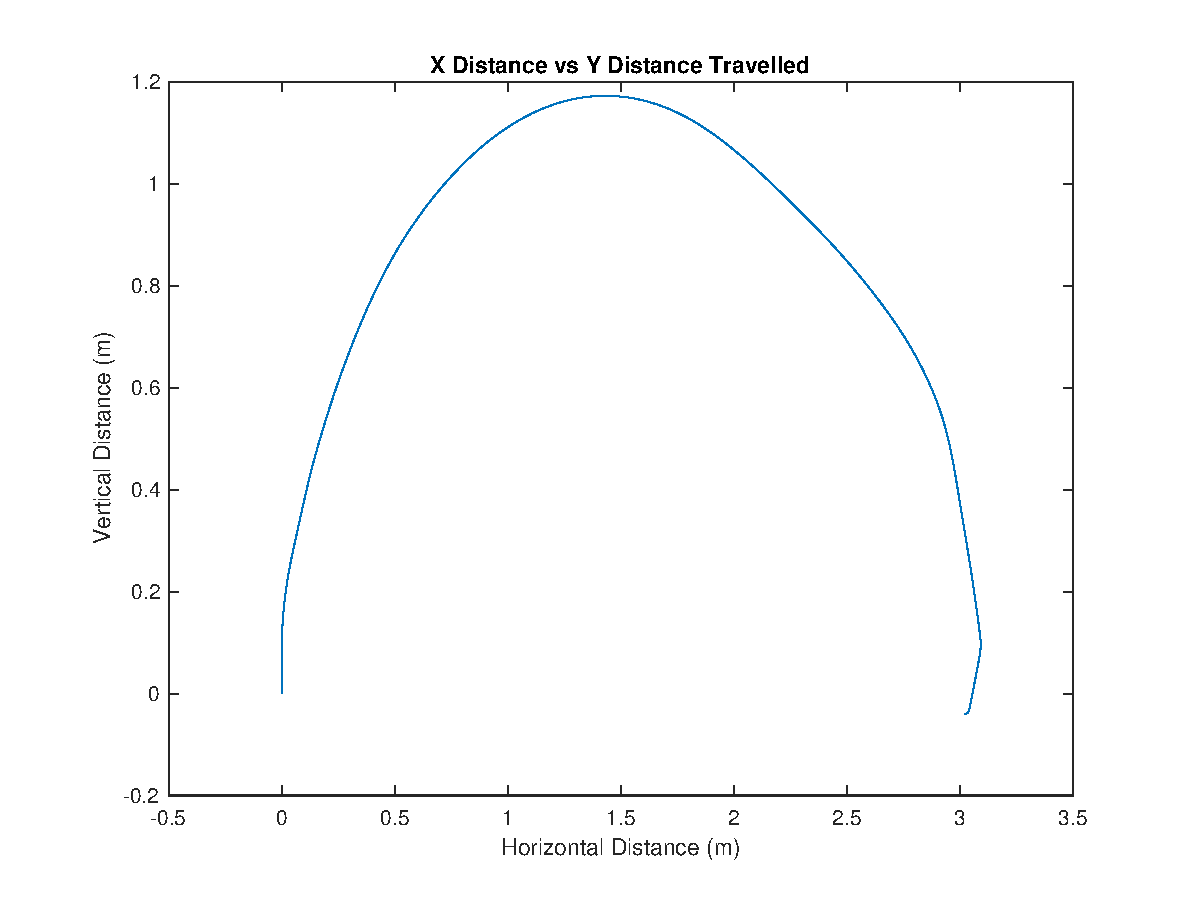
\includegraphics[scale=\bigScale]{./figures/task1_x0_y3.eps}

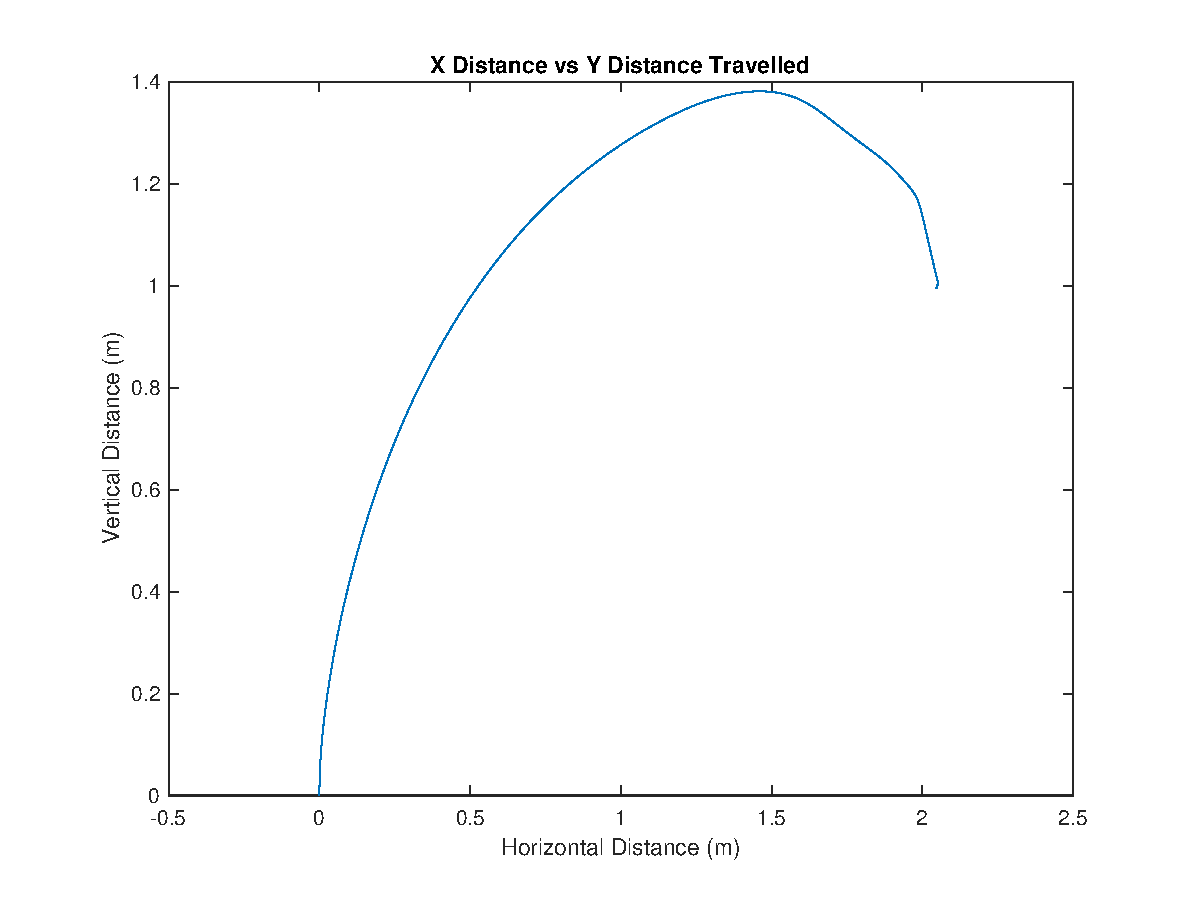
\includegraphics[scale=\bigScale]{./figures/task1_x1y2.eps}

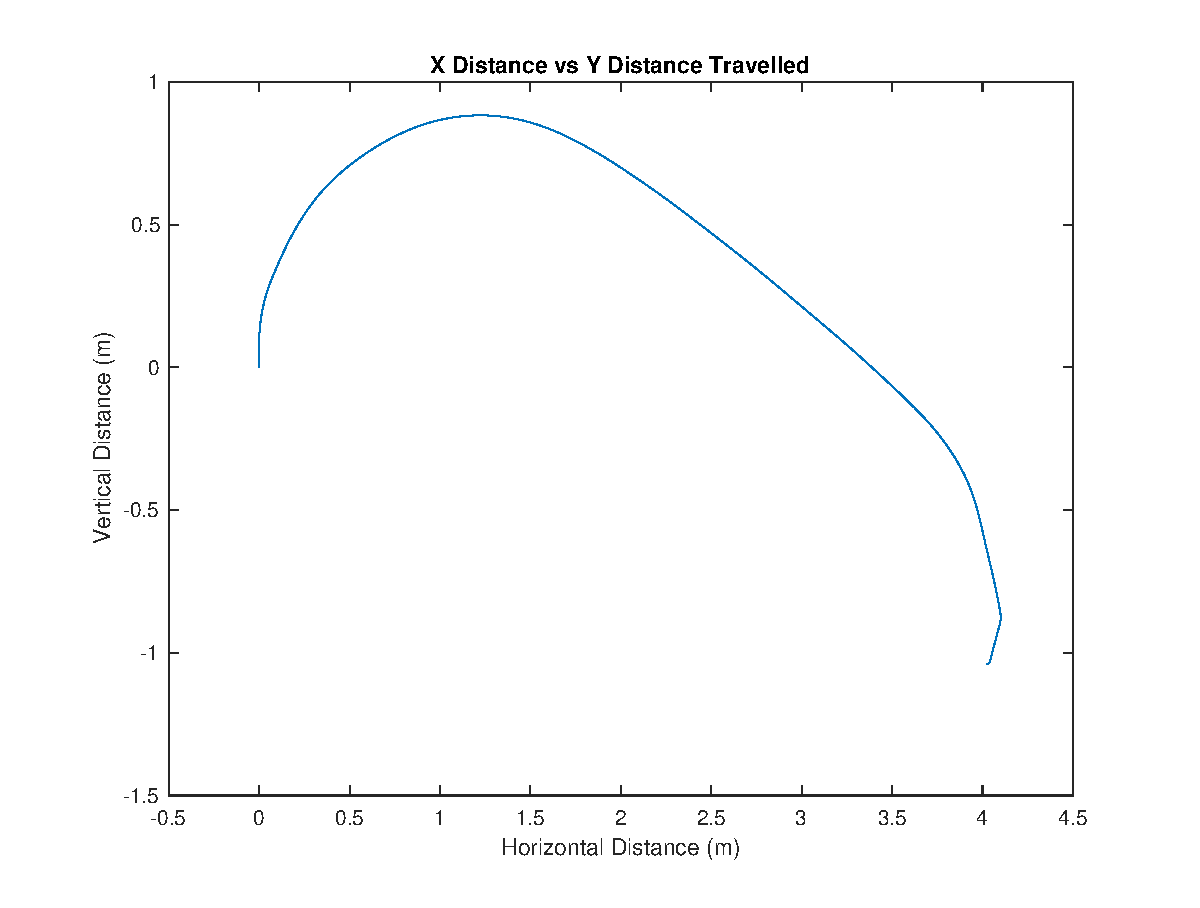
\includegraphics[scale=\bigScale]{./figures/task1_x-1y4.eps}

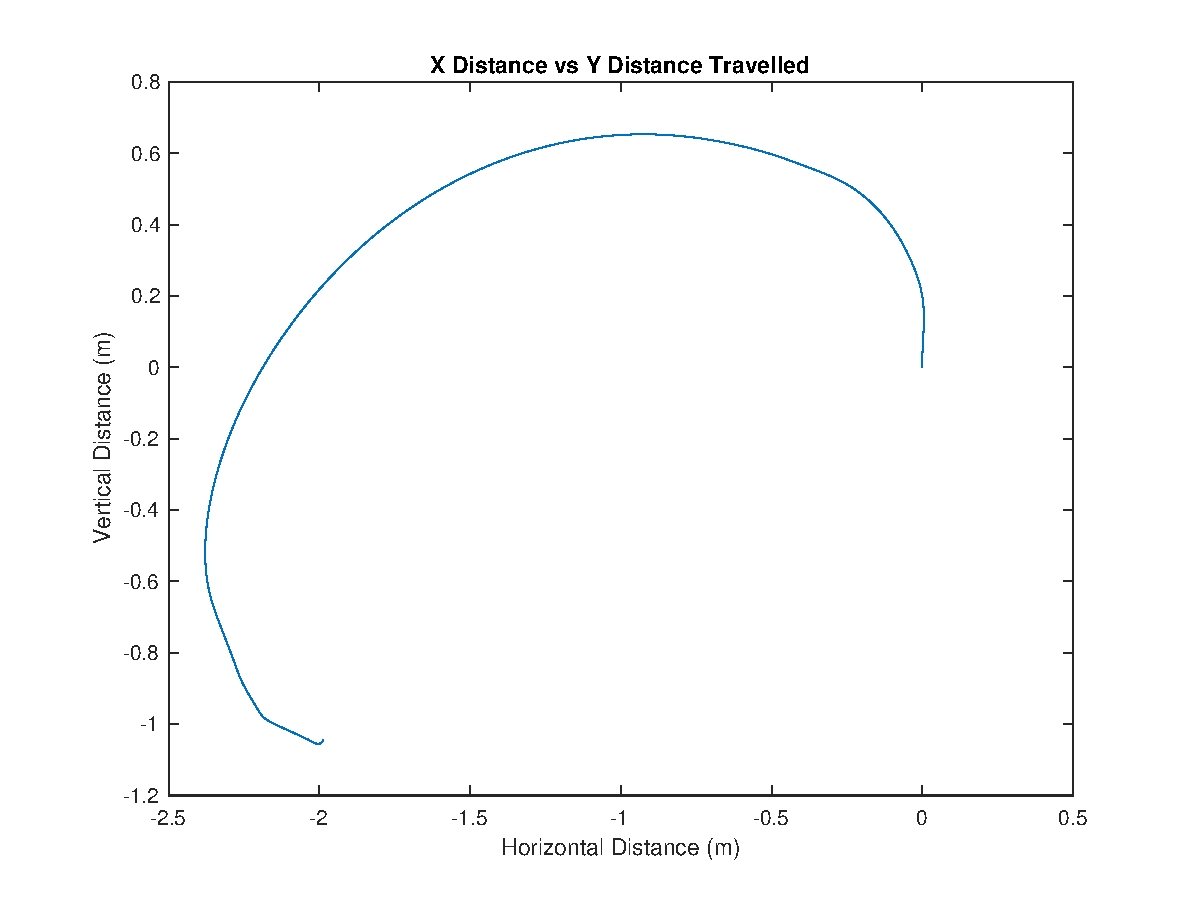
\includegraphics[scale=\bigScale]{./figures/task1_x-1y-2.eps}

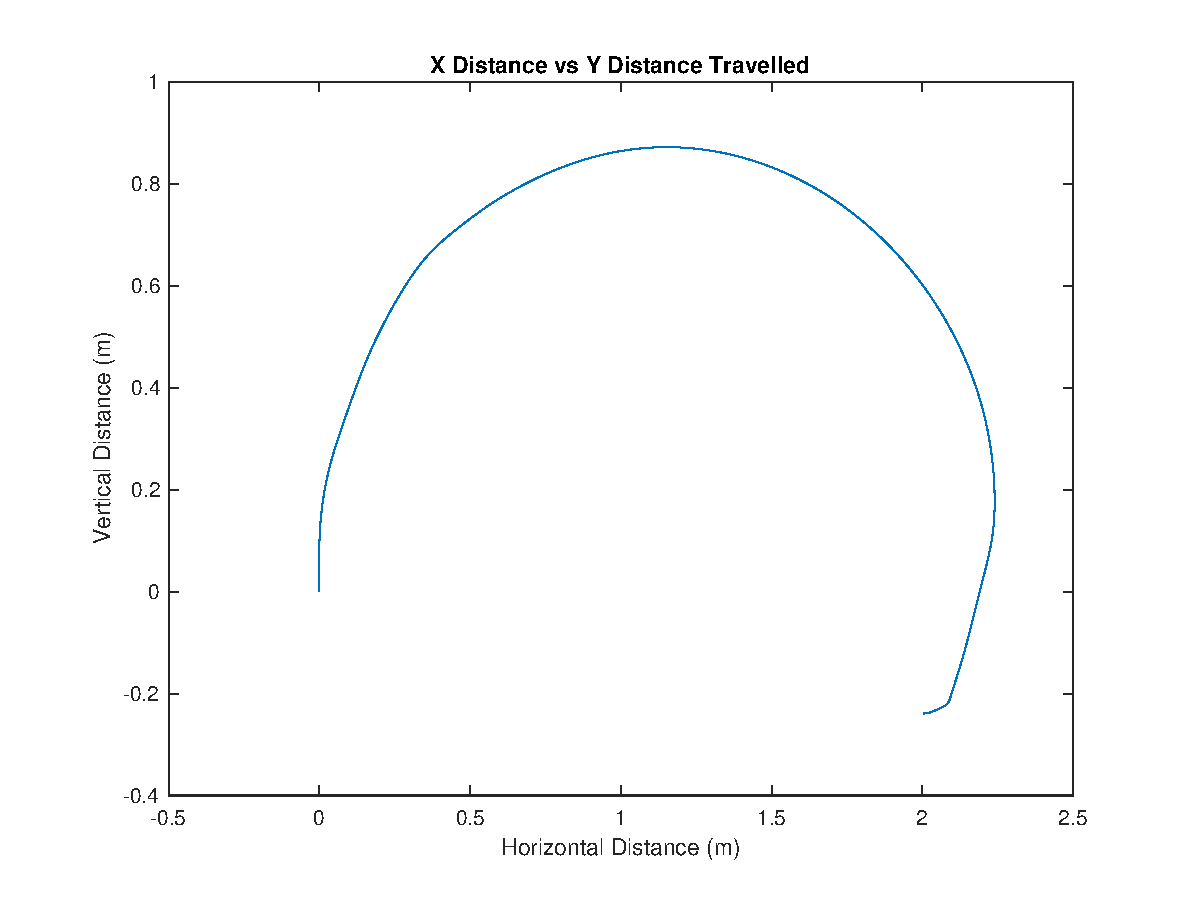
\includegraphics[scale=\bigScale]{./figures/task1_x0point2y2.eps}





\section{Path Controller Rules}
\begin{verbatim}
'1. If (psi_{ref} is S_{-ve}) and (psi is S_{-ve}) then (TurnCommand is FWD) (1) '
    '2. If (psi_{ref} is S_{-ve}) and (psi is SW) then (TurnCommand is L_{soft}) (1) '
    '3. If (psi_{ref} is S_{-ve}) and (psi is W) then (TurnCommand is L_{hard}) (1)  '
    '4. If (psi_{ref} is S_{-ve}) and (psi is NW) then (TurnCommand is L_{rot}) (1)  '
    '5. If (psi_{ref} is S_{-ve}) and (psi is N) then (TurnCommand is L_{rev}) (1)   '
    '6. If (psi_{ref} is S_{-ve}) and (psi is NE) then (TurnCommand is R_{rot}) (1)  '
    '7. If (psi_{ref} is S_{-ve}) and (psi is E) then (TurnCommand is R_{hard}) (1)  '
    '8. If (psi_{ref} is S_{-ve}) and (psi is SE) then (TurnCommand is R_{soft}) (1) '
    '9. If (psi_{ref} is S_{-ve}) and (psi is S_{+ve}) then (TurnCommand is FWD) (1) '
    '10. If (psi_{ref} is SW) and (psi is S_{-ve}) then (TurnCommand is R_{soft}) (1)'
    '11. If (psi_{ref} is SW) and (psi is SW) then (TurnCommand is FWD) (1)          '
    '12. If (psi_{ref} is SW) and (psi is W) then (TurnCommand is L_{soft}) (1)      '
    '13. If (psi_{ref} is SW) and (psi is NW) then (TurnCommand is L_{hard}) (1)     '
    '14. If (psi_{ref} is SW) and (psi is N) then (TurnCommand is L_{rot}) (1)       '
    '15. If (psi_{ref} is SW) and (psi is NE) then (TurnCommand is L_{rev}) (1)      '
    '16. If (psi_{ref} is SW) and (psi is E) then (TurnCommand is R_{rot}) (1)       '
    '17. If (psi_{ref} is SW) and (psi is SE) then (TurnCommand is R_{hard}) (1)     '
    '18. If (psi_{ref} is SW) and (psi is S_{+ve}) then (TurnCommand is R_{soft}) (1)'
    '19. If (psi_{ref} is W) and (psi is S_{-ve}) then (TurnCommand is R_{hard}) (1) '
    '20. If (psi_{ref} is W) and (psi is SW) then (TurnCommand is R_{soft}) (1)      '
    '21. If (psi_{ref} is W) and (psi is W) then (TurnCommand is FWD) (1)            '
    '22. If (psi_{ref} is W) and (psi is NW) then (TurnCommand is L_{soft}) (1)      '
    '23. If (psi_{ref} is W) and (psi is N) then (TurnCommand is L_{hard}) (1)       '
    '24. If (psi_{ref} is W) and (psi is NE) then (TurnCommand is L_{rot}) (1)       '
    '25. If (psi_{ref} is W) and (psi is E) then (TurnCommand is L_{rev}) (1)        '
    '26. If (psi_{ref} is W) and (psi is SE) then (TurnCommand is R_{rot}) (1)       '
    '27. If (psi_{ref} is W) and (psi is S_{+ve}) then (TurnCommand is R_{hard}) (1) '
    '28. If (psi_{ref} is NW) and (psi is S_{-ve}) then (TurnCommand is R_{rot}) (1) '
    '29. If (psi_{ref} is NW) and (psi is SW) then (TurnCommand is R_{hard}) (1)     '
    '30. If (psi_{ref} is NW) and (psi is W) then (TurnCommand is R_{soft}) (1)      '
    '31. If (psi_{ref} is NW) and (psi is NW) then (TurnCommand is FWD) (1)          '
    '32. If (psi_{ref} is NW) and (psi is N) then (TurnCommand is L_{soft}) (1)      '
    '33. If (psi_{ref} is NW) and (psi is NE) then (TurnCommand is L_{hard}) (1)     '
    '34. If (psi_{ref} is NW) and (psi is E) then (TurnCommand is L_{rot}) (1)       '
    '35. If (psi_{ref} is NW) and (psi is SE) then (TurnCommand is L_{rev}) (1)      '
    '36. If (psi_{ref} is NW) and (psi is S_{+ve}) then (TurnCommand is R_{rot}) (1) '
    '37. If (psi_{ref} is N) and (psi is S_{-ve}) then (TurnCommand is L_{rev}) (1)  '
    '38. If (psi_{ref} is N) and (psi is SW) then (TurnCommand is R_{rot}) (1)       '
    '39. If (psi_{ref} is N) and (psi is W) then (TurnCommand is R_{hard}) (1)       '
    '40. If (psi_{ref} is N) and (psi is NW) then (TurnCommand is R_{soft}) (1)      '
    '41. If (psi_{ref} is N) and (psi is N) then (TurnCommand is FWD) (1)            '
    '42. If (psi_{ref} is N) and (psi is NE) then (TurnCommand is L_{soft}) (1)      '
    '43. If (psi_{ref} is N) and (psi is E) then (TurnCommand is L_{hard}) (1)       '
    '44. If (psi_{ref} is N) and (psi is SE) then (TurnCommand is L_{rot}) (1)       '
    '45. If (psi_{ref} is N) and (psi is S_{+ve}) then (TurnCommand is L_{rev}) (1)  '
    '46. If (psi_{ref} is NE) and (psi is S_{-ve}) then (TurnCommand is L_{rot}) (1) '
    '47. If (psi_{ref} is NE) and (psi is SW) then (TurnCommand is L_{rev}) (1)      '
    '48. If (psi_{ref} is NE) and (psi is W) then (TurnCommand is R_{rot}) (1)       '
    '49. If (psi_{ref} is NE) and (psi is NW) then (TurnCommand is R_{hard}) (1)     '
    '50. If (psi_{ref} is NE) and (psi is N) then (TurnCommand is R_{soft}) (1)      '
    '51. If (psi_{ref} is NE) and (psi is NE) then (TurnCommand is FWD) (1)          '
    '52. If (psi_{ref} is NE) and (psi is E) then (TurnCommand is L_{soft}) (1)      '
    '53. If (psi_{ref} is NE) and (psi is SE) then (TurnCommand is L_{hard}) (1)     '
    '54. If (psi_{ref} is NE) and (psi is S_{+ve}) then (TurnCommand is L_{rot}) (1) '
    '55. If (psi_{ref} is E) and (psi is S_{-ve}) then (TurnCommand is L_{hard}) (1) '
    '56. If (psi_{ref} is E) and (psi is SW) then (TurnCommand is L_{rot}) (1)       '
    '57. If (psi_{ref} is E) and (psi is W) then (TurnCommand is L_{rev}) (1)        '
    '58. If (psi_{ref} is E) and (psi is NW) then (TurnCommand is R_{rot}) (1)       '
    '59. If (psi_{ref} is E) and (psi is N) then (TurnCommand is R_{hard}) (1)       '
    '60. If (psi_{ref} is E) and (psi is NE) then (TurnCommand is R_{soft}) (1)      '
    '61. If (psi_{ref} is E) and (psi is E) then (TurnCommand is FWD) (1)            '
    '62. If (psi_{ref} is E) and (psi is SE) then (TurnCommand is L_{soft}) (1)      '
    '63. If (psi_{ref} is E) and (psi is S_{+ve}) then (TurnCommand is L_{hard}) (1) '
    '64. If (psi_{ref} is SE) and (psi is S_{-ve}) then (TurnCommand is L_{soft}) (1)'
    '65. If (psi_{ref} is SE) and (psi is SW) then (TurnCommand is L_{hard}) (1)     '
    '66. If (psi_{ref} is SE) and (psi is W) then (TurnCommand is L_{rot}) (1)       '
    '67. If (psi_{ref} is SE) and (psi is NW) then (TurnCommand is L_{rev}) (1)      '
    '68. If (psi_{ref} is SE) and (psi is N) then (TurnCommand is R_{rot}) (1)       '
    '69. If (psi_{ref} is SE) and (psi is NE) then (TurnCommand is R_{hard}) (1)     '
    '70. If (psi_{ref} is SE) and (psi is E) then (TurnCommand is R_{soft}) (1)      '
    '71. If (psi_{ref} is SE) and (psi is SE) then (TurnCommand is FWD) (1)          '
    '72. If (psi_{ref} is SE) and (psi is S_{+ve}) then (TurnCommand is L_{soft}) (1)'
    '73. If (psi_{ref} is S_{+ve}) and (psi is S_{-ve}) then (TurnCommand is FWD) (1)'
    '74. If (psi_{ref} is S_{+ve}) and (psi is SW) then (TurnCommand is L_{soft}) (1)'
    '75. If (psi_{ref} is S_{+ve}) and (psi is W) then (TurnCommand is L_{hard}) (1) '
    '76. If (psi_{ref} is S_{+ve}) and (psi is NW) then (TurnCommand is L_{rot}) (1) '
    '77. If (psi_{ref} is S_{+ve}) and (psi is N) then (TurnCommand is L_{rev}) (1)  '
    '78. If (psi_{ref} is S_{+ve}) and (psi is NE) then (TurnCommand is R_{rot}) (1) '
    '79. If (psi_{ref} is S_{+ve}) and (psi is E) then (TurnCommand is R_{hard}) (1) '
    '80. If (psi_{ref} is S_{+ve}) and (psi is SE) then (TurnCommand is R_{soft}) (1)'
    '81. If (psi_{ref} is S_{+ve}) and (psi is S_{+ve}) then (TurnCommand is FWD) (1)'
\end{verbatim}

\end{document}
